AutoSAR是各汽车整车厂、供应商和汽车电子软件系统公司联合建立的一套协议,
旨在制定一个符合汽车电子软件开发的、开放的、标准化的软件架构。

\section{AutoSAR 架构目标}

其主要目标有三:

\begin{enumerate}
	\item 建立独立于硬件的分层软件架构
	\item 为实施应用提供方法论,包括制定无缝的软件架构堆叠流程并将应用软件整合至ECU
	\item 制定各种车辆应用接口规范,作为应用软件整合标准,以便软件构件在不同汽车平台复用
\end{enumerate}

\section{分层模型}
如图\ref{fig:AutoSAR_struct}和\ref{fig:AutoSAR_struct2},为了实现应用程序和硬件模块之间的分离,AutoSAR架构中的电子软件架构被分为四层,
从上到下依次为:应用层(Application Layer),
运行时环境(Run Time Environment,RTE),
基础软件层(Basic Software,BSW)和微控制器(Microcontroller)。

\begin{figure}[ht]
	\centering
	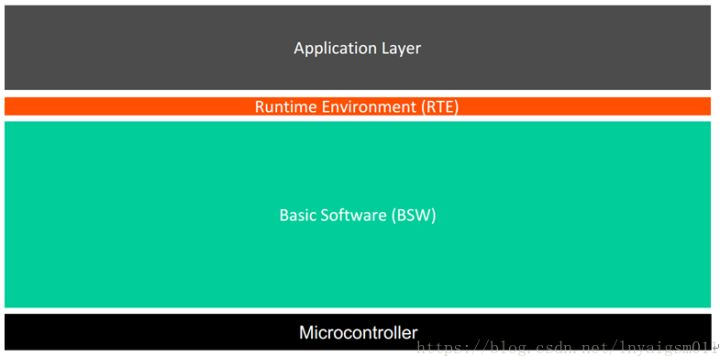
\includegraphics[scale=0.5]{./pic/autosar_struct.jpg}
	\caption{AutoSAR分层模型}
	\label{fig:AutoSAR_struct}
\end{figure}

\begin{figure}[ht]
	\centering
	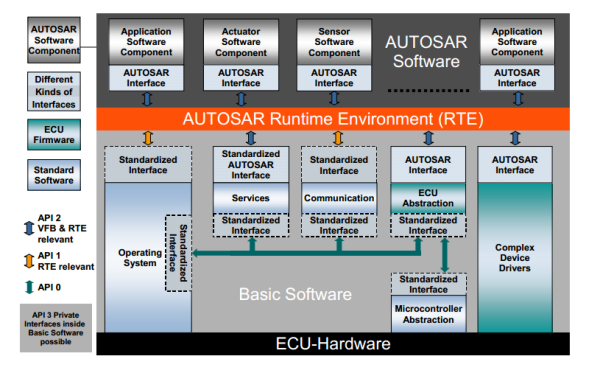
\includegraphics[scale=0.7]{./pic/autosar_struct_2.png}
	\caption{AutoSAR分层模型2}
	\label{fig:AutoSAR_struct2}
\end{figure}

\subsection{微控制器}
微控制器的底层驱动由芯片厂家提供。

\subsection{BSW}
如图\ref{fig:bsw_struct_1}BSW层可细分为:
\begin{figure}[ht]
	\centering
	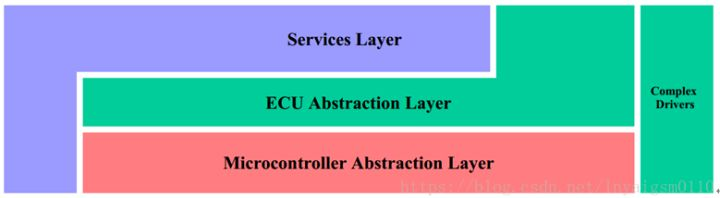
\includegraphics[scale=0.5]{pic/autosar_bsw_1.jpg}
	\caption{BSW层结构}
	\label{fig:bsw_struct_1}
\end{figure}

对于各层说明如下,具体如图\ref{fig:bsw_struct_2}所示。
\begin{figure}[ht]
	\centering
	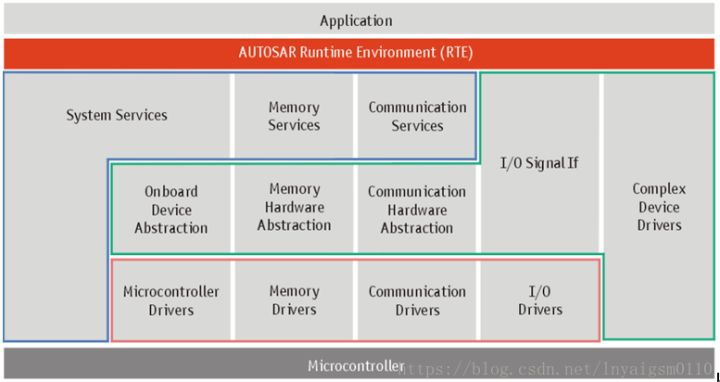
\includegraphics[scale=0.5]{pic/autosar_bsw_2.jpg}
	\caption{BSW各层结构}
	\label{fig:bsw_struct_2}
\end{figure}
\begin{enumerate}
	\item Services
	
	提供了汽车ECU非应用相关的服务,包括OS,网络通讯,内存管理(NVRAM),诊断(UDS,故障管理等),ECU状态管理模块等。
	\item ECU (Electronic Control Unit) abstraction
	
	提供了ECU应用相关的服务,它是对一个ECU的抽象,它包括了所有的ECU的输入输出,比如AD,DIO,PWM等
	\item microcontroller abstraction(MCAL)
	
	对ECU所使用的主控芯片的抽象,它跟芯片的实现紧密相关,是ECU软件的最底层部分,直接和主控芯片及外设芯片进行交互。
	\item complex drivers
	
	汽车ECU中有一些领域的ECU会处理相当复杂的硬件信号,执行相当复杂的硬件动作,例如发动机控制,ABS等,这些功能相关的软件很难抽象出来适用于所有的汽车ECU,它是跟ECU的应用以及ECU所使用的硬件紧密相关的,属于AUTOSAR构架中在不同的ECU上无法移植的部分。
\end{enumerate}

\subsection{RTE}
中间件部分给应用层提供了通信手段,这里的通信是一种广义的通讯,可以理解成接口,应用层与其他软件体的信息交互有两种,第一种是应用层中的不同模块之间的信息交互;第二种是应用层模块同基础软件之间的信息交互。而RTE就是这些交互使用的接口的集散地,它汇总了所有需要和软件体外部交互的接口。从某种意义上来看,设计符合AUTOSAR的系统其实就是设计RTE。

\subsection{应用层}
应用层中的功能由各软件组件SWC(Software Component)实现,组件中封装了部分或者全部汽车电子功能,
包括对其具体功能的实现以及对应描述,如控制大灯,空调等部件的运作,但与汽车硬件系统没有连接。
在设计开发阶段中,软件组件通信层面引入了一个新的概念,虚拟功能总线VFB(Virtual Functional Bus),
它是对AUTOSAR所有通信机制的抽象,利用VFB,开发工程师将软件组件的通信细节抽象,
只需要通过AUTOSAR所定义的接口进行描述,即能够实现软件组件与其他组件以及硬件之间的通信,
甚至ECU内部或者是与其他ECU之间的数据传输。因此软件组件只需向VFB发送输出信号,VFB将信息传输给目标组建的输入端口,
这样的方式使得在硬件定义之前,即可完成功能软件的验证,而不需要依赖于传统的硬件系统。

\subsection{术语}
\begin{enumerate}
	\item Software Component (SW-C):软件组件
	\item Virtual Functional Bus (VFB):虚拟功能总线
	\item Runtime Environment (RTE):运行环境(实时环境)
	\item Basic Software(BSW):基础软件
	\item Methodology principle:方法论原理
	\item Mode Management:模式管理
	\item Memory Abstraction:存储抽象
	\item Runnables:可运行实体
	\item MCAL:控制器抽象层
\end{enumerate}

\subsection{文档命名规则}
\begin{enumerate}
	\item EXP: 即Explaination"解释",详细介绍论题
	\item MMOD: 即Meta Model"元模型",介绍 AUTOSAR元模型
	\item MOD: 即Model"建模",介绍建模的原理
	\item RS: 即Requirement Specification"需求规范", 详细介绍需求
	\item SRS: 即Softeware Requirement Specification"软件需求规范", 描述所有软件模块的规范
	\item SWS: 即Softeware Specification"软件规范", 介绍软件模块设计和实现的规范
	\item TPS: 即Template Specification"模板规范", 详细介绍元模型
	\item TR: 即Technical Specification"技术规范",详细介绍技术规范
\end{enumerate}



